\chapter{Evaluation}
\label{chapter:evaluation}
\thispagestyle{myheadings}

% set this to the location of the figures for this chapter. it may
% also want to be ../Figures/2_Body/ or something. make sure that
% it has a trailing directory separator (i.e., '/')!
\graphicspath{{./5_Evaluation/}}
\section{Optimality checking}
Now we have learnt a model $Q_{\theta}$, we also have our test cases $\{(x_{i},y_{i})\}_{i\in[n]}$.\\
Each data window corresponds to $24$ data entries. The $t^{th}$ window corresponds to 
$$\{x_{24t}, x_{24t+1}, ..., x_{24t+23}|t\in\mathbb{I}\}$$
Each data window has $24$ data points as we have tried all possible($24$ of them) combinations of ordering of operations. For each data window we need to find the ordering of operations which requires the minimum moves according to our predictions.\\
To do this for the $t^{th}$ window of data, find the index of the minimum of $$Q_{\theta}(x_{24t}),Q_{\theta}(x_{24t+1}),...,Q_{\theta}(x_{24t+23})$$, say $k$.\\
To check if the move this corresponds to is the actual optimal move, find the index of the minimum of $y_{24t}, y_{24t+1}, ..., y_{24t+23}$, say $l$. If $k=l$ then the move we predicted as optimal is indeed optimal.\\ 
\par We train the model multiple times on the training data and measure its performance on the test data each time.\\
To measure the performance we use the predicted optimal move vs the actual optimal move.\\
\section{Results}
First, for each ordering of the operations we present the frequencies with which they are optimal in the dataset.
\begin{lstlisting}[caption=Frequencies of optimal moves in total data]
[0, 0, 0, 0, 0, 0, 0, 0, 0, 1, 0, 0, 110, 83, 84, 79, 80, 63, 307, 165, 2209, 1367, 43849, 43872]
\end{lstlisting} 
As visible the data is higly biased towards the last $2$ orderings.\\
We split this data into $70\%,30\%$ for the purpose of training and testing of our reinforcement learning agent.The random seed used resulted in the following split.
\begin{lstlisting}[caption= Frequencies of optimal move in training data]
[0, 0, 0, 0, 0, 0, 0, 0, 0, 0, 0, 0, 81, 60, 59, 54, 57, 45, 227, 119, 1526, 966, 30811, 30583]
\end{lstlisting}
\begin{lstlisting}[caption= Frequencies of optimal move in testing data]
[0, 0, 0, 0, 0, 0, 0, 0, 0, 1, 0, 0, 29, 23, 25, 25, 23, 18, 80, 46, 683, 401, 13038, 13289]
\end{lstlisting}
The predictions of our model resulted in the following $24$ true positive, False Positive, False negative and True negative results\\
\begin{lstlisting}[caption= True positives False positives False negatives True negatives]
(TP,FP,FN,TN)
(0.0, 0.0, 0.0, 27681.0)
(0.0, 0.0, 0.0, 27681.0)
(0.0, 0.0, 0.0, 27681.0)
(0.0, 0.0, 0.0, 27681.0)
(0.0, 0.0, 0.0, 27681.0)
(0.0, 0.0, 0.0, 27681.0)
(0.0, 0.0, 0.0, 27681.0)
(0.0, 0.0, 0.0, 27681.0)
(0.0, 0.0, 0.0, 27681.0)
(0.0, 0.0, 1.0, 27680.0)
(0.0, 0.0, 0.0, 27681.0)
(0.0, 0.0, 0.0, 27681.0)
(0.0, 0.0, 29.0, 27652.0)
(0.0, 0.0, 23.0, 27658.0)
(0.0, 0.0, 25.0, 27656.0)
(0.0, 0.0, 25.0, 27656.0)
(0.0, 0.0, 23.0, 27658.0)
(0.0, 0.0, 18.0, 27663.0)
(0.0, 0.0, 80.0, 27601.0)
(0.0, 0.0, 46.0, 27635.0)
(0.0, 0.0, 683.0, 26998.0)
(0.0, 0.0, 401.0, 27280.0)
(6705.0, 7667.0, 6333.0, 6976.0)
(6273.0, 7036.0, 7016.0, 7356.0)
\end{lstlisting}
So we got $12978$ predictions correct out of $27681$ test cases that is around $47\%$.
Below are 2 confusion matrices we obtained from two different runs of the predictions.\\
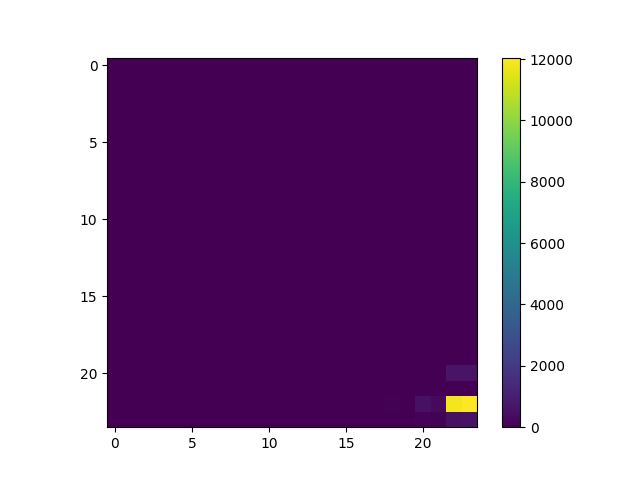
\includegraphics{cm2.png}\\
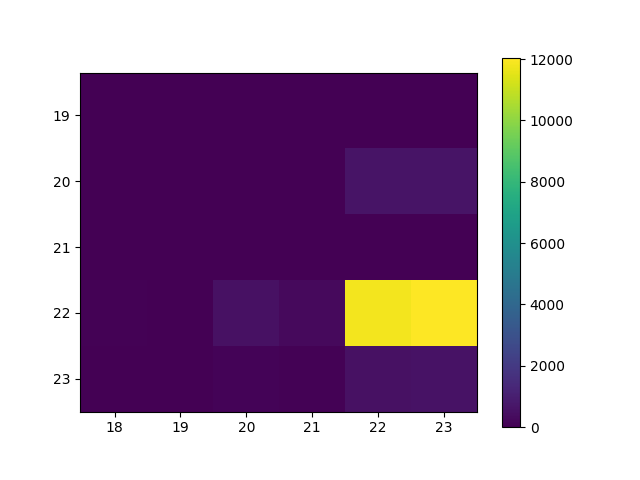
\includegraphics{cm3.png}\\
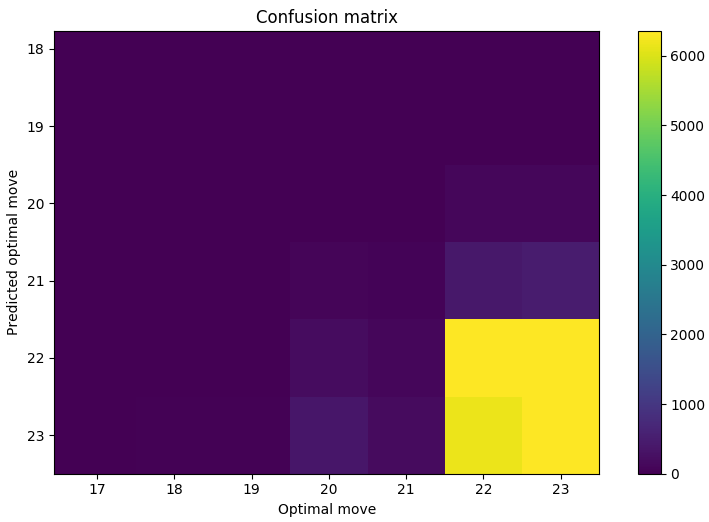
\includegraphics{cm4.png}\\
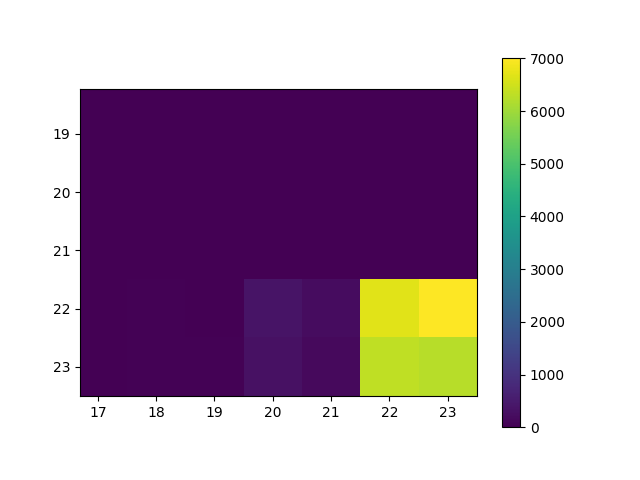
\includegraphics{cm5.png}\\
We have the actual optimal ordering, the actual worst ordering, the predicted best ordering from the model.\\
We add the number of operations required by following each of the above $3$ and look at the sum of them.\\
\begin{itemize}
    \item The sum of operations required by the optimal ordering $890640075.0$
    \item The sum of operations required by the predicted ordering $900361559.0$
    \item The sum of operations required by the optimal ordering $2310227856.0$
\end{itemize}
This tells us that our predicted orderings are approx $39\%$ of the worst ordering and $102\%$ of the best ordering.\\
A label based analysis is obtained by using $"\text{metrics.classification\_report}"$ from \\
 scikit-learn\cite{scikit-learn}.\\
\begin{lstlisting}
              precision    recall  f1-score   support

           9      0.000     0.000     0.000         1
          12      0.000     0.000     0.000        29
          13      0.000     0.000     0.000        23
          14      0.000     0.000     0.000        25
          15      0.000     0.000     0.000        25
          16      0.000     0.000     0.000        23
          17      0.000     0.000     0.000        18
          18      0.000     0.000     0.000        80
          19      0.000     0.000     0.000        46
          20      0.000     0.000     0.000       683
          21      0.000     0.000     0.000       401
          22      0.467     0.514     0.489     13038
          23      0.471     0.472     0.472     13289

   micro avg      0.469     0.469     0.469     27681
   macro avg      0.072     0.076     0.074     27681
weighted avg      0.446     0.469     0.457     27681
\end{lstlisting}

\section{Discussion}

\section{Conclusion}
%Margin fixes
%Code at end
% lstlisting has to be changed to number(caption)
%1.2 change to research problem. Most important, 1.4
%Explain and justify reinforcement learning
%What we have seen in thsi chapter, what we will see in next chapter
%Typing error, grammar
